% =====================================================================
%  Accessly – Kraków bez barier · prezentacja na HackYeah 2026
%  Maksymalnie 10 slajdów (regulamin). Każdy slajd to osobny plik w slides/.
%
%  Kompilacja (polskie znaki działają w każdym silniku):
%     latexmk main.tex                      # XeLaTeX (.latexmkrc): Atkinson Hyperlegible z fonts/ – wersja docelowa
%     latexmk -pdf main.tex                 # pdfLaTeX: zapasowo, Latin Modern
%     ./build.sh  |  ./build.sh --docker    # skrypty pomocnicze (Docker: texlive/texlive:latest-small)
%  Wersja z notatkami prelegenta:  ./build.sh --notes
% =====================================================================
\documentclass[aspectratio=169,10pt,t]{beamer}

\usepackage{iftex}
\ifPDFTeX
  \usepackage[utf8]{inputenc}
  \usepackage[T1]{fontenc}
  \usepackage{lmodern}
  \usepackage[polish]{babel}
\else
  \usepackage{fontspec}
  \usepackage{polyglossia}
  \setmainlanguage{polish}
  % Kroje (Atkinson Hyperlegible Next i Mono z fonts/) ustawia motyw: beamerthemeaccessly.sty.
\fi
\usepackage{graphicx}
\graphicspath{{img/}}
\usepackage{tabularx}
\usepackage{url}
\urlstyle{same}   % adresy tą samą czcionką co tekst
\usetheme{accessly}

\hypersetup{
  pdftitle={Accessly – Kraków bez barier (HackYeah 2026)},
  pdfauthor={Zespół Accessly},
  pdfsubject={Prototyp przewodnika po dostępnych miejscach i mapy barier},
  colorlinks=true, urlcolor=accNavy, linkcolor=accInk,
}

% ---------- Dane do uzupełnienia przed wysłaniem ----------
\newcommand{\TeamName}{Zespół Accessly}                   % nazwa zespołu
\newcommand{\TeamId}{ID zespołu: \ldots}                  % identyfikator z HackTribe
\urldef{\DemoUrl}\url{https://accessly.example.pl}        % adres działającego demo
\urldef{\RepoUrl}\url{https://github.com/HakerSII/accessly}   % repozytorium kodu
\urldef{\VideoUrl}\url{https://youtu.be/...}              % film (max 3 min, otwarte repozytorium)

\title[Accessly]{Accessly}
\subtitle[Kraków bez barier \textperiodcentered\ HackYeah 2026]{Miasto. Dostępne dla Ciebie.}
\author{\TeamName}
\date{HackYeah, 3--4 października 2026}

% ./build.sh --notes  definiuje \shownotes i dokleja notatki prelegenta po każdym slajdzie.
\ifdefined\shownotes
  \setbeameroption{show notes}
\fi

\begin{document}

% Slajd 1 – tytuł. Nazwę zespołu, ID i adresy ustawia się w main.tex.
{
\setbeamercolor{background canvas}{bg=accNavy}
\setbeamercolor{normal text}{fg=white}
\usebeamercolor[fg]{normal text}
\begin{frame}[plain]
  \vspace{6mm}
  \begin{columns}[T,onlytextwidth]
    \begin{column}{0.64\textwidth}
      \begin{tikzpicture}
        \node[fill=white,rounded corners=2.5mm,inner sep=1mm] {
\includegraphics[height=13mm]{logo}};
      \end{tikzpicture}

      \vspace{2.5mm}
      {\usebeamerfont{title}\color{white}Accessly\par}
      \vspace{0.5mm}
      {\Large\bfseries\color{white}Kraków bez barier\par}
      \vspace{2mm}
      {\color{accSignal}Twoje miasto. Twoje potrzeby. Sprawdź zanim pójdziesz.\par}
      \vspace{4mm}
      {\small\color{white}
        Przewodnik po dostępnych miejscach i~mapa barier. Każda informacja ma źródło, datę i~status weryfikacji.\par
        \vspace{3mm}
        \textbf{\TeamName}\ \textperiodcentered\ \TeamId\par
        HackYeah 2026 \textperiodcentered\ wyzwanie „Kraków bez barier” (Gmina Miejska Kraków)\par
        \vspace{2.5mm}
        {\footnotesize
        Demo: \DemoUrl\\
        Kod: \RepoUrl\\
        Film (3~min): \VideoUrl\par}}
    \end{column}
    \begin{column}{0.32\textwidth}
      \centering
      \vspace{-1mm}
      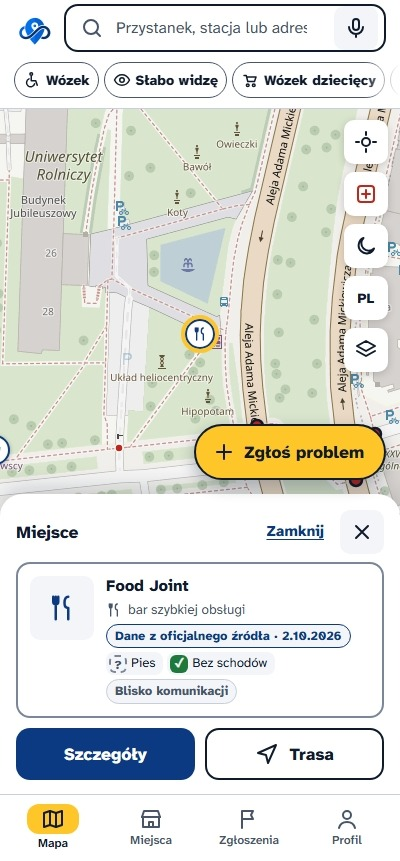
\includegraphics[height=70mm]{mobile-mapa}
    \end{column}
  \end{columns}

  \note[item]{Jedno zdanie: Accessly mówi nie „czy miejsce jest dostępne”, tylko „czy zadziała dla mnie” – i~pokazuje skąd to wiemy, od kiedy i~jak bardzo można temu ufać.}
  \note[item]{Pokazać telefon obok laptopa: ten sam prototyp działa na obu.}
  \note[item]{Nie czytać linków – są w~PDF.}
\end{frame}
}

% Slajd 2 – problem i grupa docelowa (kryterium: związek z wyzwaniem i użyteczność, 25 %).
\begin{frame}{„Dostępne / niedostępne” to za mało}
  \begin{columns}[T,onlytextwidth]
    \begin{column}{0.49\textwidth}
      \begin{block}{Problem}
        \begin{itemize}
          \item Jedna etykieta nie mówi, czy wjadę z~wózkiem, czy drzwi mają 90~cm, czy jest toaleta i~gdzie można odpocząć.
          \item Informacje w~sieci nie mają źródła ani daty: zepsuta winda zamienia „dostępne” w~zmarnowaną wyprawę.
          \item Brak informacji bywa pokazywany tak, jakby był jej potwierdzeniem.
          \item Miasto nie ma zasobów, by ręcznie utrzymywać bazę -- dane muszą aktualizować się same.
        \end{itemize}
      \end{block}
    \end{column}
    \begin{column}{0.49\textwidth}
      \begin{block}{Dla kogo -- zakres prototypu}
        \begin{itemize}
          \item \textbf{Grupa główna:} osoby poruszające się na wózkach oraz rodzice z~wózkami dziecięcymi (profile „Wózek” i~„Wózek dziecięcy”).
          \item Te same dane obsługują kolejne profile: Słabo widzę, Senior, Po zabiegu (turystyka medyczna), Bagaż, Podróżuję z~psem, Rower.
          \item Mieszkańcy i~turyści (interfejs PL, EN, DE, UK) oraz \textbf{właściciele i~zarządcy obiektów}, którzy dostają własny panel.
        \end{itemize}
      \end{block}
    \end{column}
  \end{columns}
  \vspace{2mm}
  \begin{exampleblock}{Nasza odpowiedź}
    Accessly odpowiada na pytanie \textbf{„czy to miejsce zadziała dla mnie?”} konkretnymi faktami o~barierach
    i~udogodnieniach. Każdy fakt ma \textbf{źródło, datę i~status weryfikacji}, a~brak danych jest pokazany
    jako brak danych -- nigdy jako dostępność.
  \end{exampleblock}

  \note[item]{Zacząć od historii: Anna na wózku chce wyjść na kawę w~centrum. Mapa z~zeszłego roku mówi „dostępne”, a~dziś przy wejściu jest próg i~nikt nie wie, czy toaleta jest na dole.}
  \note[item]{Podkreślić dwie grupy: użytkownicy końcowi oraz właściciele – bez nich dane nie będą aktualne.}
  \note[item]{Profil to preferencje (schody, winda, cisza), nie informacja o~niepełnosprawności – wraca na slajdzie o~prywatności.}
\end{frame}

% Slajd 3 – co prototyp już robi (kryterium: jakość i kompletność prototypu, 20 %).
\begin{frame}{Działający prototyp: aplikacja webowa na telefon i~komputer}
  \begin{columns}[T,onlytextwidth]
    \begin{column}{0.57\textwidth}
      \small
      \begin{itemize}
        \item \textbf{Katalog 6\,545 miejsc} Krakowa (OpenStreetMap) w~7~kategoriach
              i~\textbf{27 atrybutów}: schody, podjazd, winda, drzwi $\geq$~90~cm, toaleta, przewijak,
              pętla indukcyjna, miejsca odpoczynku, parking OzN w~pobliżu, cisza, pies\ldots
        \item \textbf{Profil potrzeb} zamiast pytania o~niepełnosprawność: filtruje, sortuje,
              oznacza „Dopasowane do Ciebie” i~mówi, czego brakuje.
        \item \textbf{Karta miejsca:} każda informacja ze źródłem, datą i~statusem; Aktualne / Nieaktualne /
              Popraw / Uzupełnij, pytanie do właściciela, opinie, zdjęcia, trasa dla wózka.
        \item \textbf{Mapa barier} („Yanosik dostępności”): 10 typów zgłoszeń, waga (blokuje / utrudnienie),
              głosy „nadal jest” / „naprawione”, automatyczne wygasanie.
        \item \textbf{Asystent w~języku naturalnym} (Claude z~narzędziem wyszukiwania w~bazie; bez klucza --
              reguły słów kluczowych). Pokazuje wyłącznie fakty z~bazy.
        \item \textbf{11 warstw otwartych danych}, panel właściciela, panel administratora,
              4~języki, tryb dzienny i~nocny.
      \end{itemize}
    \end{column}
    \begin{column}{0.41\textwidth}
      \screenshot{mapa-desktop}
      \vspace{0.5mm}
      \muted{Mapa z~profilem „Wózek”: miejsca (grupowane), warstwy miasta i~OSM, zgłoszone bariery
        z~wagą i~liczbą potwierdzeń. Lista obok mapy to jej tekstowa alternatywa.}
      \vspace{2mm}

      \kpi{6\,545}{miejsc z~OSM}\hfill\kpi{11}{warstw danych}\hfill\kpi{503}{testów automatycznych}
    \end{column}
  \end{columns}

  \note[item]{To nie makieta: wszystko na slajdzie działa w~repozytorium (Python stdlib + czysty JS, bez zależności).}
  \note[item]{Dane o~miejscach z~OSM: 1\,495 z~6\,545 miejsc ma już co najmniej jeden atrybut dostępności; reszta ma „brak danych” – i~tak to pokazujemy.}
  \note[item]{Asystent AI jest opcjonalny; w~kontenerze demo działa tryb reguł, więc nic nie zależy od sieci.}
\end{frame}

% Slajd 4 – mapa demonstracji na żywo (pkt 6 wyzwania: określić potrzeby grupy, sprawdzić miejsce,
% pokazać konkretne bariery i udogodnienia, źródło i datę informacji, oznaczenie danych niepełnych
% i przykładowych). Scenariusz kończy się sukcesem: Anna znajduje miejsce, które spełnia wszystkie jej potrzeby.
% Slajd wisi na ekranie tuż przed przejściem do aplikacji; szczegóły w notatkach.
\begin{frame}{Demo: Anna na wózku znajduje restaurację bez barier}
  \begin{columns}[T,onlytextwidth]
    \begin{column}{0.63\textwidth}
      \scriptsize
      \renewcommand{\arraystretch}{1.1}
      \begin{tabularx}{\textwidth}{@{}>{\bfseries\color{accNavy}}c >{\raggedright\arraybackslash}p{30mm} >{\raggedright\arraybackslash}X@{}}
        \toprule
        & \textbf{Krok} & \textbf{Na co zwrócić uwagę} \\
        \midrule
        1 & Preferencje: bez schodów, toaleta dostępna, parking OzN &
            mapa i~listy pokazują tylko bariery ważne dla Anny; miejsca posortowane według dopasowania \\
        2 & Pytanie: „restauracja na Kazimierzu bez schodów, z~toaletą i~parkingiem” &
            ranking z~uzasadnieniem: Kuchnia u~Doroty na górze spełnia wszystko; przy innych widać, czego \emph{nie wiadomo} \\
        3 & Karta miejsca: Kuchnia u~Doroty &
            zielone „Spełnia wszystkie Twoje potrzeby”; każdy fakt ze źródłem, datą i~statusem; braki nazwane wprost \\
        4 & Po drodze: zgłoszenie „Brak windy” na przystanku, waga „blokuje” &
            kwadrat = blokuje; głosy „nadal jest” / „naprawione”; awaria wygasa po 14~dniach \\
        5 & Panel właściciela: „Potwierdź informacje” &
            status „Potwierdzone przez właściciela”; Anna dostaje powiadomienie \\
        \bottomrule
      \end{tabularx}

      \vspace{1.5mm}
      \textbf{Przypadki brzegowe w~demo:} dane sprzeczne $\rightarrow$ „Wymaga ponownej weryfikacji”;
      dane miasta niedostępne $\rightarrow$ snapshot z~datą „stan na”; brak informacji nigdy nie znaczy „dostępne”.

      \vspace{1mm}
      \muted{Dane przykładowe są oznaczone: konta demo (\texttt{anna@}, \texttt{kasia@}, \texttt{admin@accessly.test}),
        zgłoszenia testowe, etykieta „Tryb demo”.}
    \end{column}
    \begin{column}{0.35\textwidth}
      \screenshot{asystent-ok-wynik}\par
      \vspace{0.3mm}
      \muted{Krok 2: miejsce, które spełnia wszystko -- zielone znaczniki i~„Dopasowane do Ciebie”.}
      \vspace{1.5mm}
      \screenshot{karta-ok-atrybut}\par
      \vspace{0.3mm}
      \muted{Krok 3: jeden fakt -- wartość, źródło, data, status i~przyciski Aktualne / Nieaktualne / Popraw.}
    \end{column}
  \end{columns}

  \note[item]{Czas: ok. 3 minuty. Przed wejściem: aplikacja na telefonie i~laptopie, mapa na Kazimierzu, w~Profilu zaznaczone preferencje bez schodów, toaleta dostępna, parking OzN (bez chipa „Wózek”: wymaga on też szerokości drzwi, której nie ma w~danych OSM, więc dawałby „Spełnia 2~z~3”), panel właścicielki otwarty w~drugiej karcie.}
  \note[item]{Krok 1 (0:00–0:30): pokazać Profil $\rightarrow$ „Moje preferencje” i~listę „Najbliżej środka mapy”; miejsca z~odznaką „Dopasowane do Ciebie” są wyżej.}
  \note[item]{Krok 2 (0:30–1:00): zakładka Miejsca, wpisać „Restauracja na Kazimierzu bez schodów, z~dostępną toaletą i~parkingiem” – w~trybie reguł wynik jest deterministyczny: „Znalazłem 535 pasujących miejsc; 1~z~pokazanych spełnia wszystkie Twoje wymagania”, na górze Kuchnia u~Doroty.}
  \note[item]{Krok 3 (1:00–1:45): otworzyć kartę; zielona ramka; pokazać palcem trzy rzeczy przy atrybucie: źródło, datę, status. Przewinąć do atrybutu bez danych (np. szerokie drzwi) – nasz najważniejszy komunikat: nie zgadujemy. Przyciski Aktualne / Nieaktualne / Popraw, „Uzupełnij” i~pytanie do właściciela.}
  \note[item]{Krok 4 (1:45–2:20): „Zgłoś problem”, pinezka na przystanku Stradom, typ „Brak windy”, waga „blokuje”; pokazać kształt znacznika (kwadrat = blokuje) i~głosy. Zgłoszenie można zrobić bez konta.}
  \note[item]{Krok 5 (2:20–3:00): w~drugiej karcie \texttt{/owner.html} jako \texttt{kasia@accessly.test} (Camelot Cafe) kliknąć „Potwierdź informacje”; wrócić do karty tego lokalu – status się zmienił.}
  \note[item]{Przypadki brzegowe (gdy jury pyta lub zostaje czas): chip „Wózek” i~„Spełnia 2~z~3, brak danych: szerokie drzwi”; historia atrybutu ze sprzecznymi głosami; strona „Źródła danych” z~datami snapshotów.}
  \note[item]{Jeśli padnie sieć: wszystko poza kafelkami mapy działa z~danych lokalnych. Dane przykładowe: trzy konta demo i~zgłoszenia testowe; widok administratora bez logowania ma etykietę „Tryb demo: dane przykładowe”.}
\end{frame}

% Slajd 5 – źródła danych, aktualność, wiarygodność (kryterium: wiarygodność oraz sposób prezentacji i aktualizacji danych, 15 %).
\begin{frame}{Dane, którym można zaufać}
  \begin{columns}[T,onlytextwidth]
    \begin{column}{0.49\textwidth}
      \begin{block}{3 źródła informacji}
        \begin{itemize}
          \setlength{\itemsep}{0.3mm}
          \item \textbf{Open Data \& OSM}\\
                Dane publiczne i~otwarte
          \item \textbf{Property Owner}\\
                Potwierdzone informacje bezpośrednio od właściciela obiektu
          \item \textbf{Community}\\
                Użytkownicy potwierdzają, poprawiają i~uzupełniają dane
        \end{itemize}
      \end{block}
    \end{column}
    \begin{column}{0.49\textwidth}
      \begin{block}{Każdy fakt ma kontekst}
        \centering\textbf{Źródło \textperiodcentered\ Data \textperiodcentered\ Status weryfikacji}\par
      \end{block}
      \vspace{1mm}
      \begin{exampleblock}{Accessly Trust Model}
        \pill{accNavy}{Owner verified} $\rightarrow$ \pill{accOk}{Community confirmed} $\rightarrow$\\[0.8mm]
        \pill{accNavy}{Official source} $\rightarrow$ \pill{accMuted}{Unverified}
        \begin{itemize}
          \setlength{\itemsep}{0pt}
          \item nieaktualne dane są oznaczane,
          \item sprzeczności są widoczne,
          \item brak informacji nigdy nie oznacza „dostępne”.
        \end{itemize}
      \end{exampleblock}
    \end{column}
  \end{columns}

  \note[item]{Przypadek testowy wymagany w~wyzwaniu – dane sprzeczne: właściciel mówi „bez schodów”, dwie osoby zgłaszają „nieaktualne” $\rightarrow$ status „Wymaga ponownej weryfikacji”, wartość zostaje z~ostrzeżeniem, obie strony widać w~historii.}
  \note[item]{Przypadek – źródło niedostępne: usługa ArcGIS miasta nie odpowiada $\rightarrow$ aplikacja pokazuje warstwę ze snapshotu z~datą „stan na”; żaden ekran nie jest pusty.}
  \note[item]{Przypadek – dane niepełne: „Spełnia 1~z~3 Twoich potrzeb, brak danych: szerokie drzwi” – miejsce nie dostaje odznaki „Dopasowane do Ciebie”.}
  \note[item]{Sprawdziliśmy też GTFS Krakowa i~dane.gov.pl: pola o~dostępności są puste, nikt nie publikuje awarii wind – dlatego awarie pochodzą ze zgłoszeń.}
\end{frame}

% Slajd 6 – architektura i skalowanie (kryteria: potencjał wdrożeniowy i skalowanie, 20 %; RULES: Design / Technical).
\begin{frame}{Architektura: pozyskiwanie danych oddzielone od prezentacji}
  \centering
  \begin{tikzpicture}[x=1mm,y=1.32mm,
      box/.style={draw=accLineStrong,fill=accSoft,rounded corners=1.2mm,text width=23mm,align=center,
                  font=\fontsize{6.3}{7.6}\selectfont,execute at begin node={\hyphenpenalty=10000},
                  inner sep=1mm,minimum height=8.5mm},
      tall/.style={box,minimum height=42mm},
      head/.style={font=\scriptsize\bfseries,text=accNavy,anchor=south},
      ext/.style={draw=accLineStrong,dashed,fill=white,rounded corners=1.2mm,text width=142mm,align=center,
                  font=\fontsize{6.3}{7.6}\selectfont,execute at begin node={\hyphenpenalty=10000},
                  inner sep=1.2mm},
      arr/.style={-{Stealth[length=1.5mm]},accNavy,line width=0.5pt},
      both/.style={{Stealth[length=1.5mm]}-{Stealth[length=1.5mm]},accNavy,line width=0.5pt}]
    % nagłówki kolumn
    \node[head] at (12.5,46.5) {ŹRÓDŁA};
    \node[head] at (42,46.5) {POZYSKANIE I~AKTUALIZACJA};
    \node[head] at (72,46.5) {MAGAZYN};
    \node[head] at (102,46.5) {API JSON};
    \node[head] at (131.5,46.5) {PREZENTACJA};
    % kolumna 1: źródła
    \node[box] (s1) at (12.5,42) {OpenStreetMap (ODbL)};
    \node[box] (s2) at (12.5,33.5) {Otwarte dane Krakowa (ArcGIS)};
    \node[box] (s3) at (12.5,25) {Właściciele obiektów};
    \node[box] (s4) at (12.5,16.5) {Społeczność: potwierdzenia, poprawki, zgłoszenia barier};
    % kolumna 2: pozyskanie
    \node[box] (i1) at (42,42) {\texttt{build\_osm\_*.py} $\rightarrow$ snapshoty w~\texttt{data/}};
    \node[box,minimum height=8mm] (i2) at (42,33) {\texttt{layers.py}: pobieranie stronami, pamięć podręczna 24~h, odświeżanie w~tle};
    \node[box,minimum height=12mm] (i3) at (42,20.5) {\texttt{api.py}: zmiany właścicieli, poprawki i~głosy, moderacja; każda zmiana trafia do historii};
    % kolumna 3: magazyn
    \node[tall] (db) at (72,29) {\textbf{SQLite} (biblioteka standardowa)\\[0.8mm]miejsca \textperiodcentered\ atrybuty: wartość, źródło, data, potwierdzenia, zaprzeczenia \textperiodcentered\ historia \textperiodcentered\ zgłoszenia barier i~głosy \textperiodcentered\ konta i~role \textperiodcentered\ zdjęcia\\[0.8mm]migracje wersjonowane, WAL, transakcje};
    % kolumna 4: API
    \node[tall] (api) at (102,29) {\textbf{\texttt{server.py} / \texttt{api.py}}\\[0.8mm]\texttt{/api/places} (profil $\rightarrow$ dopasowanie, status)\\\texttt{/api/layers} \textperiodcentered\ \texttt{/api/reports}\\\texttt{/api/ai} \textperiodcentered\ \texttt{/api/route}\\\texttt{/api/owner} \textperiodcentered\ \texttt{/api/admin}\\[0.8mm]limity rozmiaru, gzip, role};
    % kolumna 5: prezentacja
    \node[box] (p1) at (131.5,42) {Aplikacja web (telefon i~komputer), 4~języki};
    \node[box] (p2) at (131.5,33.5) {Panel właściciela};
    \node[box] (p3) at (131.5,25) {Panel administratora};
    \node[box] (p4) at (131.5,16.5) {Klienci API (planowane Open API): miasto, mapy, rezerwacje};
    % strzałki
    \draw[arr] (s1) -- (i1);
    \draw[arr] (s2) -- (i2);
    \draw[arr] (s3.east) -- (i3.west |- s3.east);
    \draw[arr] (s4.east) -- (i3.west |- s4.east);
    \draw[arr] (i1.east) -- (db.west |- i1.east);
    \draw[arr] (i2.east) -- (db.west |- i2.east);
    \draw[arr] (i3.east) -- (db.west |- i3.east);
    \draw[both] (db) -- (api);
    \draw[both] (api.east |- p1.west) -- (p1.west);
    \draw[both] (api.east |- p2.west) -- (p2.west);
    \draw[both] (api.east |- p3.west) -- (p3.west);
    \draw[arr] (api.east |- p4.west) -- (p4.west);
    % usługi opcjonalne
    \node[ext] at (72,6.5) {\textbf{Usługi opcjonalne, każda z~działaniem zastępczym:} Claude API (rekomendacje; bez klucza -- reguły słów kluczowych) \textperiodcentered\ OpenRouteService (trasy dla wózka) \textperiodcentered\ Nominatim (wyszukiwanie z~przeglądarki, tylko po zatwierdzeniu) \textperiodcentered\ backend Rampa (zgłoszenia barier przez adapter \texttt{api.js})};
  \end{tikzpicture}

  \note[item]{Najważniejsze zdanie: import i~odświeżanie danych są osobnym krokiem (skrypty, snapshoty, cache), a~prezentacja czyta tylko z~bazy przez API – można podmienić frontend albo źródło bez ruszania reszty.}
  \note[item]{Backend Rampa (FastAPI, PostgreSQL, model obserwacja $\rightarrow$ głos $\rightarrow$ zaufanie) powstał równolegle; adapter w~\texttt{api.js} pozwala przenieść zgłoszenia barier tam bez zmian w~aplikacji. To ścieżka skalowania na większe wdrożenie.}
  \note[item]{Uczciwie: konfiguracja warstw miejskich jest dziś w~kodzie (\texttt{layers.py}), nie w~pliku miasta – to pierwszy krok przy drugim mieście.}
\end{frame}

% Slajd 7 – dostępność cyfrowa: wykaz funkcji dostępnych i elementów do dalszych prac (pkt 5 i 6 wyzwania).
\begin{frame}{Dostępność cyfrowa: WCAG 2.2 AA jako cel, główny scenariusz już sprawdzony}
  \begin{columns}[T,onlytextwidth]
    \begin{column}{0.63\textwidth}
      \begin{block}{Jest w~prototypie (kontrola głównego scenariusza: klawiatura, czytnik ekranu, kontrast, mapa jako tekst)}
        \footnotesize
        \begin{itemize}
          \item \textbf{Klawiatura:} każda akcja to przycisk lub link; link „Przejdź do treści”; widoczny fokus;
                fokus nie ginie, gdy listy odświeżają się co 15~s; Esc zamyka panele.
          \item \textbf{Czytnik ekranu:} landmarki i~nagłówki, etykiety ARIA, krótkie komunikaty „live” zamiast czytania
                całych list; mapa ma opis odsyłający do listy tekstowej; tytuł okna zmienia się z~widokiem.
          \item \textbf{Mapa w~formie tekstu:} listy Zgłoszenia, Miejsca i~najbliższych obiektów warstw jako przyciski;
                waga problemu kształtem i~podpisem (kwadrat / koło), nie tylko kolorem.
          \item \textbf{Kontrast i~czytelność:} tokeny kolorów 4,5:1 (tekst) i~3:1 (kontrolki, symbole) -- test liczy je
                ze \texttt{style.css}; tryb nocny; czcionka Atkinson Hyperlegible; 4~języki.
          \item \textbf{Formularze i~dotyk:} błędy w~\texttt{role="alert"} z~nazwą brakującego pola, „Dalej” nigdy
                nie jest zablokowane; cele $\geq$~44~px; układ działa do 400\,\% powiększenia.
        \end{itemize}
      \end{block}
    \end{column}
    \begin{column}{0.35\textwidth}
      \begin{alertblock}{Do dalszych prac}
        \footnotesize
        \begin{itemize}
          \item Audyt całego scenariusza z~NVDA / VoiceOver i~testy z~użytkownikami na wózkach i~słabowidzącymi.
          \item Nawigacja klawiaturą po znacznikach mapy (Leaflet) i~alternatywa dla ustawiania pinezki
                przez przesuwanie mapy (kryterium 2.5.7).
          \item Panele właściciela i~administratora w~tym samym standardzie.
          \item Formalna deklaracja dostępności i~raport zgodności.
        \end{itemize}
      \end{alertblock}
      \vspace{1mm}
      \muted{Zmiany z~ostatnich dwóch iteracji („WCAG 2.2 A”, „WCAG 2.2 AA”) są objęte testami
        \texttt{AccessibilityTests} w~repozytorium.}
    \end{column}
  \end{columns}

  \note[item]{Pokazać na żywo: Tab przez listę zgłoszeń, Enter otwiera szczegóły, Esc wraca; przełączyć tryb nocny.}
  \note[item]{„Tekstowa alternatywa mapy” to wymaganie wprost z~wyzwania – u~nas lista obok mapy jest pierwszorzędnym widokiem, nie dodatkiem.}
  \note[item]{Nie mówić „jesteśmy zgodni z~WCAG”; mówić „główny scenariusz spełnia kryteria A/AA, które sprawdziliśmy, a~tu jest lista braków”.}
\end{frame}

% Slajd 8 – ochrona danych i bezpieczeństwo oraz uruchomienie i utrzymanie poza UMK (pkt 5 wyzwania).
\begin{frame}{Prywatność, bezpieczeństwo i~utrzymanie poza infrastrukturą UMK}
  \begin{columns}[T,onlytextwidth]
    \begin{column}{0.5\textwidth}
      \begin{block}{Dane użytkowników i~bezpieczeństwo}
        \footnotesize
        \begin{itemize}
          \item \textbf{Bez konta:} mapa, katalog i~zgłaszanie barier -- anonimowo; serwer nie zapisuje adresów IP
                ani identyfikatorów urządzeń.
          \item \textbf{Profil potrzeb = preferencje} (schody, winda, cisza), nigdy diagnoza ani informacja
                o~niepełnosprawności; zapisany w~przeglądarce, z~kontem -- także na serwerze.
          \item \textbf{Konto bez hasła:} e-mail + jednorazowy kod (15~min, 5~prób); kody i~tokeny tylko jako skróty
                SHA-256; ciasteczko HttpOnly, SameSite, Secure; usunięcie konta jednym przyciskiem.
          \item \textbf{Serwer:} HTTPS (Caddy, Let's Encrypt), limity rozmiaru żądań (10~kB, zdjęcia 4~MB),
                treści użytkowników zawsze escapowane (testy), role sprawdzane przy każdym żądaniu.
          \item Polityka prywatności i~lista ciasteczek w~aplikacji; zapytania do asystenta AI nie są logowane.
        \end{itemize}
      \end{block}
    \end{column}
    \begin{column}{0.5\textwidth}
      \begin{block}{Uruchomienie i~utrzymanie -- propozycja}
        \footnotesize
        \begin{itemize}
          \item \textbf{Operator:} zespół Accessly (spółka lub fundacja) albo partner społeczny; UMK bez obowiązku
                utrzymywania bazy i~bez dostępu do systemów wewnętrznych.
          \item \textbf{Hosting (szacunek):} jeden VPS w~UE (2~vCPU, 4~GB) ok.~60--120~zł/mies., domena, poczta
                transakcyjna; asystent AI rozliczany od zapytania (ułamki grosza); mapa z~OSM.
          \item \textbf{Aktualizacje:} jedno polecenie (\texttt{scripts/deploy.sh}, Ansible); dane miasta odświeżają się
                same co 24~h, OSM skryptem (zalecane co miesiąc); kopie zapasowe SQLite \texttt{.backup}.
          \item \textbf{Zgłoszenia i~moderacja:} kolejka w~panelu administratora (przejęcia lokali, poprawki,
                nowe miejsca, konta właścicieli), powiadomienia e-mail, statystyki brakujących danych.
          \item \textbf{Przenośność:} Docker + Ansible na dowolną infrastrukturę; licencje otwarte
                (ODbL, BSD, PSF, Apache) wymienione w~aplikacji.
        \end{itemize}
      \end{block}
    \end{column}
  \end{columns}

  \note[item]{Pytanie jury „jakie dane zbieracie?”: bez konta – żadnych; z~kontem – e-mail, opcjonalna nazwa, profil potrzeb. Tabela w~polityce prywatności w~aplikacji.}
  \note[item]{RODO: profil potrzeb to świadoma decyzja projektowa – wyzwanie wprost prosi, by nie wymagać informacji o~niepełnosprawności.}
  \note[item]{Kwoty to szacunki na podstawie cenników VPS; nie obiecywać konkretnego dostawcy.}
\end{frame}

% Slajd 9 – model biznesowy i komercjalizacja (kryterium: 20 %; pkt 9 wyzwania).
\begin{frame}{Model biznesowy: bezpłatne dla mieszkańców, płatne dla obiektów i~miast}
  \small
  \renewcommand{\arraystretch}{1.25}
  \begin{tabularx}{\textwidth}{@{}>{\bfseries\raggedright\arraybackslash}p{3.3cm} X >{\raggedright\arraybackslash}p{3.6cm}@{}}
    \toprule
    Segment & Oferta & Przychód \\
    \midrule
    Mieszkańcy i~turyści & aplikacja, profil potrzeb, asystent, mapa barier & bezpłatnie -- zawsze; to oni tworzą dane, które napędzają resztę \\
    Właściciele obiektów (hotele, gastronomia, kultura, sieci) & panel podstawowy bezpłatny; \textbf{plan Pro}: odznaka „Potwierdzone przez właściciela”, statystyki „czego szukają goście, czego brakuje”, hurtowe dodawanie udogodnień, widget dostępności na stronę i~do systemu rezerwacji & abonament za obiekt lub pakiet dla sieci \\
    Organizatorzy wydarzeń, zarządcy nieruchomości & pakiet czasowy: tymczasowe wejścia i~trasy, mapa barier na czas imprezy, komunikacja z~uczestnikami & opłata za wydarzenie / obiekt \\
    Miasta i~regiony & wdrożenie white-label (konfiguracja, import OSM, warstwy miejskie), raporty „gdzie brakuje danych i~udogodnień” do planowania & wdrożenie + roczne utrzymanie \\
    Dostawcy map, aplikacji turystycznych, systemów rezerwacyjnych & Open API z~atrybucją: fakty o~dostępności ze źródłem, datą i~statusem & licencja API / limity zapytań \\
    \bottomrule
  \end{tabularx}

  \vspace{2.5mm}
  \begin{exampleblock}{Zasady, które chronią wartość danych}
    Nie sprzedajemy danych osobowych. Treści społeczności i~dane z~OSM pozostają otwarte (ODbL, atrybucja zachowana).
    Właściciel płaci za narzędzia i~widoczność, nie za „lepszy” status -- status zawsze wynika z~weryfikacji.
  \end{exampleblock}

  \note[item]{Najbardziej realny pierwszy przychód: hotele i~turystyka medyczna (profil „Po zabiegu”, warstwa SOR / apteki, 4~języki) – goście zza granicy pytają o~dostępność przed rezerwacją.}
  \note[item]{Panel właściciela już dziś pokazuje „Najczęściej wyszukiwane informacje o~Twoim lokalu” – to zalążek statystyk z~planu Pro.}
  \note[item]{Miasto nie jest klientem w~pierwszej kolejności; korzysta z~danych i~raportów, a~ewentualnie finansuje wdrożenie white-label.}
\end{frame}

% Slajd 10 – od prototypu do usługi: co jest, co dalej, warunki kolejnego miasta (pkt 6 wyzwania).
\begin{frame}{Od prototypu do usługi}
  \begin{columns}[T,onlytextwidth]
    \begin{column}{0.44\textwidth}
      \begin{exampleblock}{Mamy dziś}
        \footnotesize
        \begin{itemize}
          \item Działający prototyp na telefon i~komputer: 6\,545 miejsc, 27 atrybutów, 11 warstw danych,
                mapa barier, asystent, 4~języki.
          \item Panel właściciela (potwierdzanie, pytania, zdjęcia, udogodnienia hurtowo)
                i~panel administratora (kolejka, statystyki, braki danych).
          \item Źródło, data i~status przy każdej informacji; brak danych pokazany jako brak.
          \item Główny scenariusz zgodny z~WCAG 2.2 A/AA w~sprawdzonych kryteriach.
          \item 503 testy, Docker, Ansible, HTTPS, polityka prywatności.
        \end{itemize}
      \end{exampleblock}
    \end{column}
    \begin{column}{0.54\textwidth}
      \begin{block}{Plan na 3--6 miesięcy}
        \footnotesize
        \begin{enumerate}
          \item \textbf{Pilotaż} z~organizacją osób z~niepełnosprawnościami, 2--3 hotelami i~instytucjami kultury;
                audyt dostępności z~użytkownikami.
          \item \textbf{Produkcyjne logowanie} (poczta transakcyjna, opcjonalnie OAuth), powiadomienia, tryb offline (PWA).
          \item \textbf{Weryfikacja ze zdjęć i~tekstu z~pomocą AI} -- jako propozycje do potwierdzenia, nigdy jako fakty;
                silnik zaufania z~backendu Rampa.
          \item \textbf{Open API i~widget} dla właścicieli; integracja z~systemami rezerwacyjnymi.
          \item \textbf{Drugie miasto:} konfiguracja + wyciąg OSM + warstwy miejskie w~pliku miasta.
                Warunek: otwarte dane miasta (lub sam OSM) i~lokalny partner do moderacji.
        \end{enumerate}
      \end{block}
    \end{column}
  \end{columns}
  \vspace{2mm}
  \centering
  {\large\bfseries\color{accNavy}Nie budujemy kolejnej statycznej mapy.
   Budujemy żywy, weryfikowalny obraz dostępności miasta -- z~mieszkańcami, właścicielami i~otwartymi danymi.\par}
  \vspace{1.5mm}
  \muted{Demo: \DemoUrl\ \textperiodcentered\ Kod: \RepoUrl\ \textperiodcentered\ Film: \VideoUrl}

  \note[item]{Zakończyć zdaniem z~tego slajdu i~zaprosić do stolika z~telefonem – niech jury samo kliknie „Zgłoś problem”.}
  \note[item]{Pytanie o~zespół po hackathonie: operator (spółka / fundacja), moderacja w~panelu, finansowanie z~planu Pro i~wdrożeń white-label.}
\end{frame}


\end{document}
